\documentclass{article}
\usepackage[margin=1.5in]{geometry}

\usepackage{graphicx}
\graphicspath{ {C:/Users/Programming/Documents/ML/Kaggle/Titanic/} }

\title{Study of Titanic Data Set}
\date{2017-10-01}
\author{Samuel Ruckley Jones}


\begin{document}
\pagenumbering{gobble}
\maketitle
\newpage
\pagenumbering{arabic}

\section{Abstract}
This article documents some  manipulations of the Kaggle Titanic data set with the aim of exploring how these manipulations effect different prediction models. A concentration is put on the encoding of non-numeric variables and the effectiveness of correlated integer encoding. 
\newpage
\section{Introduction}

This document gives a summary of the main data manipulation techniques that were used to change the prediction accuracy on the Kaggle Titanic Data set. A full description of all the steps and the code used to implement them can be seen in the Titanic.pyc file. The main aim of this project was to teach the author how to use the sci-kit learn and numpy packages of python and some general data manipulation techniques and so has been written more as a record of steps taken than a paper. However, there may be some interesting notes for those new to machine learning. The concentration of this project was to see how data manipulation can effect prediction models rather than too achieve the highest possible prediction accuracy, however, the most succesfull manipulations were combined to achieve a 3-4\% improvment in detection accuracy.
\linebreak
\linebreak
During this project the following was implemented:

\begin{itemize}
\item The basics of the python programming language
\item Data manipulation using numpy
\item Employing built in machine learning techniques using scikit-learn
\item Data manipulation techniques including
\begin{itemize}
\item Non-numeric data encoding (Integer Encoding, One-Hot encoding)
\item Handeling missing data
\item Variable transformation
\item Creating new variables
\item Normalisation and Standardisation
\end{itemize}
\end{itemize}

\newpage
\subsection{Summary of Data Set}

The Titanic data set is made up of attributes of the passengers on the titanic. The goal is to predict which of these passengers survived with the highest possible prediction accuracy.
The titanic data set contains the following variables:

\begin{itemize}
\item PassengerId: Assending numbering of passengers
\item Pclass: The class of the passenger (1, 2, 3)
\item Name: Passenger Name
\item Sex: Passenger Sex, Male or Female
\item Age: Passenger Age
\item SibSp: The number of Siblings or spouses the passenger has on board the ship
\item Parch: The number of parents or children the passenger has on the ship
\item Ticket: Ticket of the passenger, sometimes non-numeric
\item Fare: The price paid by the passenger
\item Cabin: The cabin number the passenger stayed in
\item Embarked: The port the passenger embarked, C = Cherbourg, Q = Queenstown, S = Southampton
\end{itemize}

\subsection{Testing Process}

Predictor training was performed using built in machine learning models from scikit-learn. After each manipulation of the data set a spot check was used to identify any changes to the prediction accuracy when compared to the baseline results. For each model K-fold cross validation (CV) is performed and the average of the K feature weight sets is used to find the new prediction accuracy for that model. The random seed used by sci-kit learn for non-deterministic models is kept constant so that results are comparable. While not shown in this document, to check that results were not effected by unstable predictors, the random seed was changed to different values and all tests re-run. All results remained within a 1\% margin at all tested random seeds.
\linebreak
The prediction models used for testing were:
\begin{itemize}
\item Linear Regression (LR)
\item Linear Discriminant Analysis (LDA)
\item K-Nearest Neighbors (KNN)
\item Classification and Regression Trees (CART)
\item Naive Bayesian (NB)
\item Support Vector Machines (SVM)
\end{itemize}

\newpage

\section{Initial Data Analysis and Pre-Processing}

A data set which is used for prediction should have a roughly equal split between classes. If this is not the case the developed prediction algorithm is likely to show bias. For this reason the percentage of examples who survived was calculated and came out to 38\%. This is close enough to a 50:50 split to prevent Bias.

A spot check was needed to get a baseline for the accuracy of each algorithm. As many ML algorithms require numeric and or complete data sets, some pre-processing was needed.
\linebreak
The following data manipulations were performed:
\begin{itemize}
\item PassengerId is just sequential numbering of examples and so was dropped
\item The 'Age' variable is missing from 20\% of the examples. This is relatively small percentage and easy to interporlate so missing ages were replaced with the average age
\item The 'Name' and 'Ticket' variables may contain data but are non-numeric and difficult to transform so were dropped from baseline test
\item The 'Cabin' variable was missing from 77\% of the examples. This is a large amount of missing data from a hard to interpolate variable and so 'Cabin' was dropped
\item The 'Embarked' variable was missing from 0.2\% of the examples. This only accounted for 2 examples and so these examples were dropped
\end{itemize}


\subsection{Normalisation}
After transformation all data is normalized using a min-max scaler. This ensures all variables are in the same order of magnitude. This prevents certain variables from having an added weight i.e, if not normalized Passenger age may have a larger sway on the prediction than Sex than it should do due most of its variables being an order of magnitude larger. Normalization is performed before each spot check.
\par
Standardisation could also be applied to the data. This changes all variables to have a mean of 0 and a standard deviation of 1. It assumes that all variables have a bell curve distribution which is not neccisarily true and so was not perfromed during this project. However, it can help some models that assume variables have a standard distribution such as LR and LDA and so may be added to this project in the future.

\newpage
\subsection{Baseline Predictions}

A spot check was performed to get an idea of what algorithms work best with the data set. The results of this spot check are used to compare the effects of any changes performed on the data set. They also allowed the author to see how certain algorithms are more sensitive to certain types of data manipulation.
\linebreak
Initial prediction results:

\begin{itemize}
\item LR: 0.801839 (0.045890)
\item LDA: 0.794777 (0.039523)
\item KNN: 0.811620 (0.042290)
\item CART: 0.787715 (0.041363)
\item NB: 0.800430 (0.049380)
\item SVM: 0.787774 (0.054174)
\end{itemize}

\newpage
\section{Detailed Pre-Processing}

To improve prediction accuracy the variables of the data set were analysed in more detail. Transformations to the data were then performed to increase or the amount of usable information available to the prediction algorithms. In this section the transformation that produced the largest change in accuracy or which produced interesting results are highlighted.

\subsection{Non-numeric Variable Encoding}

In order to allow prediction algorithms to be run on the data set non-numeric data must be encoded. This is normally performed using integer encoding or one hot encoding.
\par 
Integer encoding (IE) replaces each class of the variable with an integer. For example in the Embarked class C, Q and S are replaced with 1, 2 and 3. This is the simplest form of encoding and works relatively well. However it can cause problems as it introduces a mathematical relationship between classes that should not exist. In this example a prediction algorithm could now interpret S = C + Q.
\par 
During this project an encoding technique that will be named Correlated Integer Encoding was also experimented with. This is identical to IE but the variable class that best correlates with the target is given the encoding 1, the second most 2 and so on. In this project that would mean the variable class that has the highest survival rate would be encoded with 1, the next with 2 and so on.
\par
One-hot encoding solves the mathematical relationship problem by including a new variable for each class of the original variable. For example Embarked would be replaced with 3 variables, C, Q and S. A passenger embarking from Queenstown would have a 0 for variables C and S and a 1 for Q. This encoding tends to perform better but can greatly increase the processing power needed to create a prediction algorithm.

\subsection{Passenger Name}
A passengers name doesn't provide any particular information about there chances of survival, however, their title does indicate their level of wealth and influence which would effect their chances. For this reason a new variable called "Title" was extracted from the name variable. To prove the hypothesis the percentage survival rates for each title were plotted:
\par
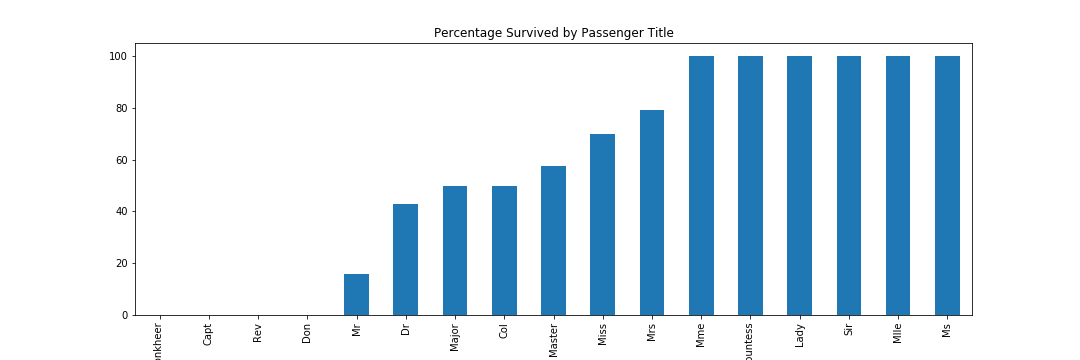
\includegraphics[width=\textwidth]{Percentage_Survived_by_Passenger_Title}
\par
From this figure it is obvious to see that there is a correlation between Survival and Title. It also provides some information that was not previously in the data set. For example it seems that a "Mrs" is slightly more likely to survive than a "Mrs", splitting the examples down further than the "Sex" variable.
\par
The "Title" data set needs to be encoded to be used. The 3 different encoding techniques described above were used and the effect on predictor accuracy compared. The following plots show the change in accuracy from the baseline.
\par
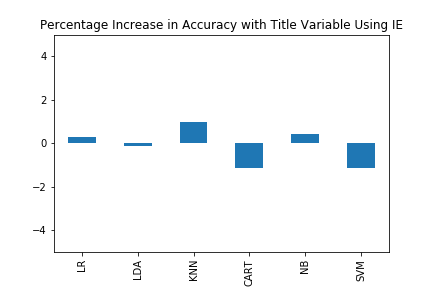
\includegraphics[width=5cm, height=4cm]{Percentage_Increase_in_Accuracy_with_Title_Variable_Using_IE}
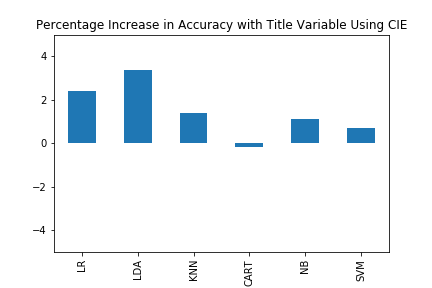
\includegraphics[width=5cm, height=4cm]{Percentage_Increase_in_Accuracy_with_Title_Variable_Using_CIE}
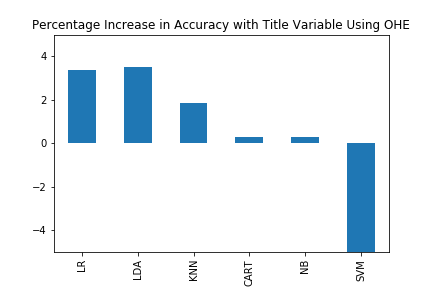
\includegraphics[width=5cm, height=4cm]{Percentage_Increase_in_Accuracy_with_Title_Variable_Using_OHE}
\par
It can be seen that including passenger title variable increases predictor accuracy with the exception of CART and NB. As expected OHE improves predictor accuracy in comparison with IE. However, the interesting result is that CIE and OHE have comparable effects on accuracy which suggests that in some cases CIE can improve accuracy without the computational intensity of OHE. The large drop in NB accuracy is due to NB algorithm assuming that all variables are completely uncorrelated and OHE causes a variable to be split into many entirely co-linear variables.
\par
\subsection{Passenger Age}
As the policy in emergency marine situations is "Women and Children First" it would be reasonable to assume that children would have a higher survival rate than adults and so the Age variable would effect the prediction accuracy. To Prove this Hypothesis the survival rate of each age was plotted. Both plots show the same data but the second shows the ages grouped in 2 year splits as it makes patterns slightly easier to observe.
\par
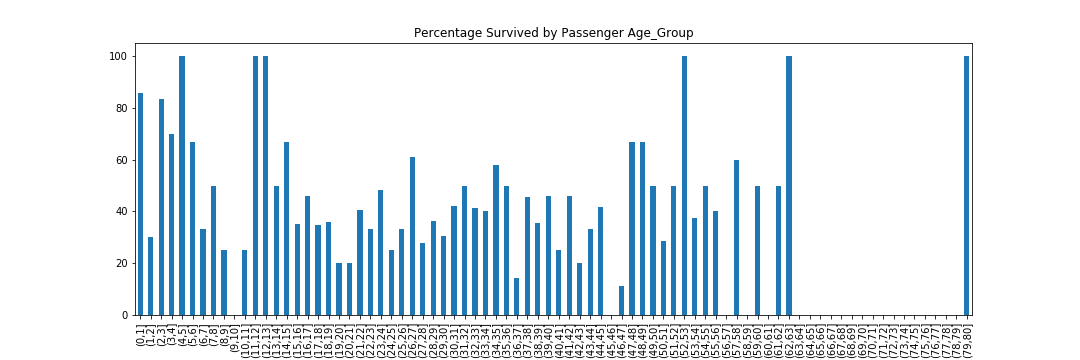
\includegraphics[width=\textwidth]{Percentage_Survived_by_Passenger_Age_Group}
\par
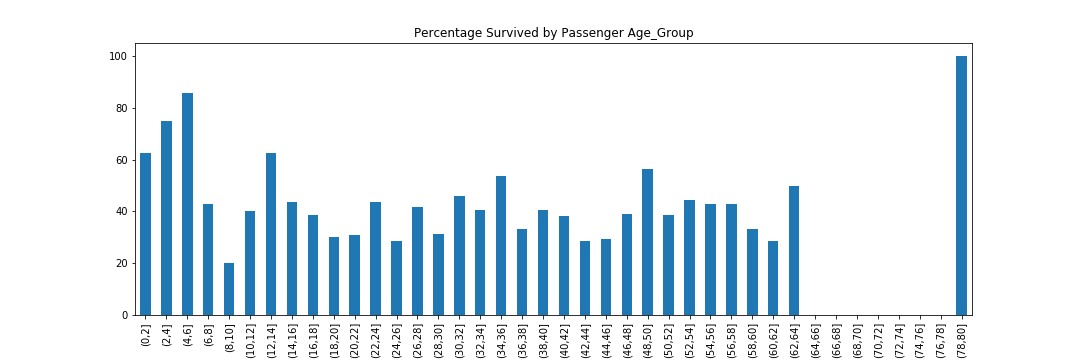
\includegraphics[width=\textwidth]{Percentage_Survived_by_Passenger_Age_Group_increment_2}
\par
It can be seen that survival chance does increase for young children but interestingly there is a dip in survival rate for 8-10 year olds. After a quick analysis it can be seen that most children were in the 3rd class so one theory to explain this dip as small children could have been ferried to life boats but larger children would have been trapped at lower levels with the adults and had less physical ability to get to safety. This also means that the age-survival relationship is not entirely positive which may have effects on model accuracy
\par
Bellow is a plot of the change in accuracy of each model when the age variable is removed
\par
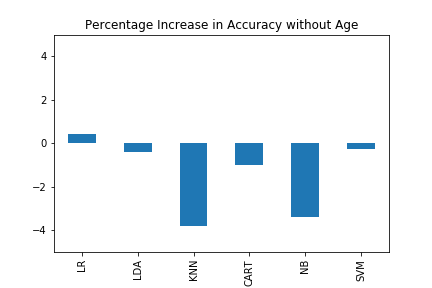
\includegraphics[width=5cm, height=4cm]{Percentage_Increase_in_Accuracy_without_Age}
\par
It can be seen that Age actually has very little effect on accuracy for many of the models. The models that were effected were KNN and SVM, which may have been better at expressing the non positive Age-Survival relationship.
\par
As CIE and OHE caused an increase in accuracy for the Title variable it was decided to try it hear. To do this each age was considered a group, as in the plots above, and each group given an encoding. The results of this encoding are shown below:
\par
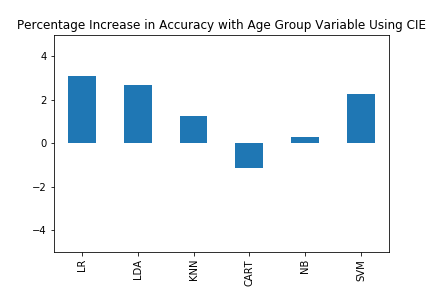
\includegraphics[width=5cm, height=4cm]{Percentage_Increase_in_Accuracy_with_Age_Group_Variable_Using_CIE}
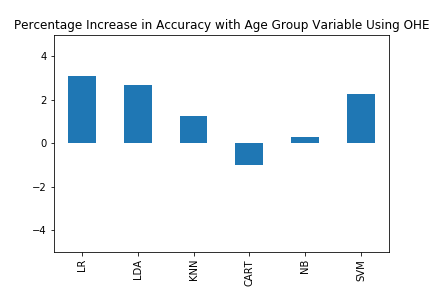
\includegraphics[width=5cm, height=4cm]{Percentage_Increase_in_Accuracy_with_Age_Group_Variable_Using_OHE}
\par
It can be seen that both encoding methods have an effect on all models. It can be seen that the models that see the largest increase such as LR, LDA and SVM are the ones that where originally unaffected by the removal of the age variable. This suggests that this new encoding has allowed these models to make use of the information held in the original age variable. This may be expected for OHE but it is also true for CIE which suggests that encoding raw data can in some cases increase the amount of usable information.
\par
\subsection{Ticket}
The ticket variable may hold valuable information for predictors, however, in its raw state is is unusable as it is a non-numeric variable with no separate classes to group into. The ticket values can be split into a Prefix string and a number. The number always starts with the passenger class which provides no new information and there is no obvious information provided my the rest of the number. For this reason it was decided to use the prefixes to see if they provide any new information. Any Tickets that did not have a prefix were given a placeholder prefix 'U'. The following plot shows the percentage survival rate for each prefix.
\par
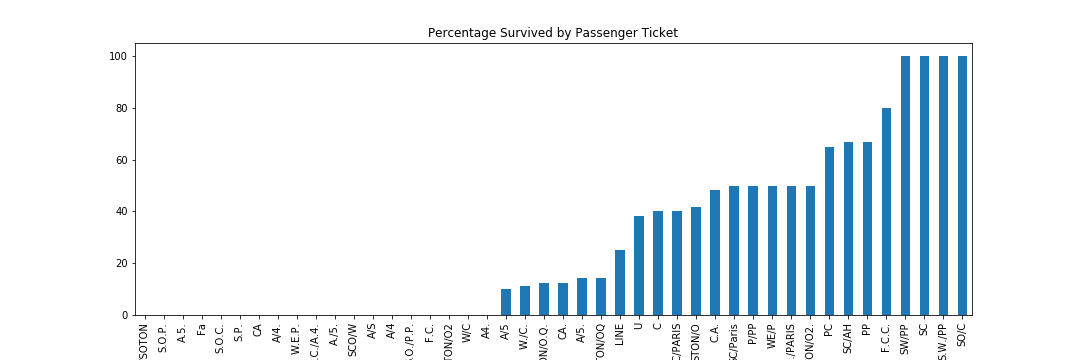
\includegraphics[width=\textwidth]{Percentage_Survived_by_Passenger_Ticket}
\par
It can be seen that there is definitely some correlation between certain ticket prefixes and survival. The effects on model accuracy using encoded prefixes are shown below:
\par
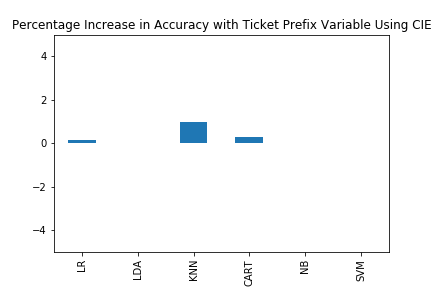
\includegraphics[width=5cm, height=4cm]{Percentage_Increase_in_Accuracy_with_Ticket_Prefix_Variable_Using_CIE}
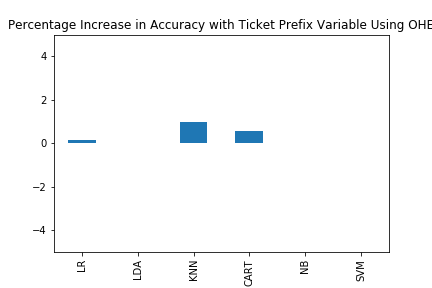
\includegraphics[width=5cm, height=4cm]{Percentage_Increase_in_Accuracy_with_Ticket_Prefix_Variable_Using_OHE}
\par
These show very little change in performance. This may be because much of the information provided by the prefixes is already encompassed in other variables. However, it may also be due to the poor quality of prefix class distribution. For example more than half of the prefixes only contain 100\% or 0\% survival cases. This will introduce a large amount of bias into this variable which will hurt its effect on accuracy.
\subsection{Combining Transformations}
Combining the transformations detailed above using CIE resulted in the following results:

\begin{itemize}
\item LR: 0.836718 (0.052193)
\item LDA: 0.831084 (0.057553)
\item KNN: 0.807218 (0.039660)
\item CART: 0.804441 (0.038264)
\item SVM: 0.819836 (0.059212)
\item NB: 0.814182 (0.055762)
\end{itemize}
\par
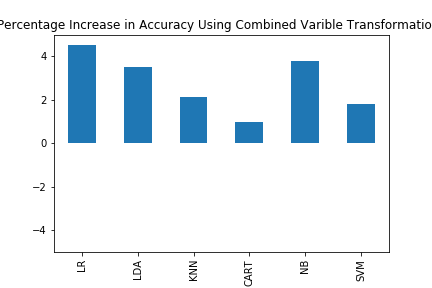
\includegraphics[width=5cm, height=4cm]{Percentage_Increase_in_Accuracy_Using_Combined_Varible_Transformations}
These results show a general improvement across all models with a maximum detection accuracy from LR of 83.6\%

\section{Conclusion}
This project has shown examples of how manipulating a data set can increase a predictors accuracy. It has been shown that transforming a variable can increase the amount of information available such as in the Name and Ticket cases. It has been shown that encoding a variable in a different way can increase a predictors accuracy such as in the Age case.
\par
The most intriguing thing to me while manipulating this data set is how effective CIE could be at increasing model accuracy such as in the Age case. The best explanation I can think of for this effect is that correlating the variable with survival reduces the complexity models need to express the title to survival relationship. For example, after CIE the titile-survival correlation is entirely positive which is simpler for LR to express using theta*(variable value). CIE was not always effective, when used on SibSp or Parch (not detailed here) it resulted in a small negative change which suggests that it may only be useful on certain variables or possibly that it works better on variables with a large number of classes. It is also interesting how CIE produced very similar results to OHE in some cases which suggests it may be a good way of reducing computational complexity in some cases. This test case is obviously not large enough to make any concrete conclusions, however, I will keep CIE in mind for future projects.
\par
There is obviously a lot more room to manipulate this data set to improve prediction accuracy, this may be attempted in the future.





\end{document}


